\documentclass[../../informe/src/main.tex]{subfiles}

\begin{document}

Se desea realizar un circuito que convierta un número binario de 4 bits en su complemento a dos.

%empiezo a enumerar subítems de consigna.
\begin{enumerate}

%item 1, expresión como suma de mintérminos. Presento notación.
\item Expresamos el valor de cada bit de salida en función de los mintérminos de los bits de entrada.\par
Sean $b_{3}$, $b_{2}$, $b_{1}$ y $b_{0}$ los bits de entrada, donde $b_{3}$ es el bit más significativo y $b_{0}$ el menos significativo.\par
A su vez, sean $y_{3}$, $y_{2}$, $y_{1}$ e $y_{0}$ los bits de salida (complemento a dos de la entrada), donde $y_{3}$ es el bit más significativo e $y_{0}$ el menos significativo. \par
Luego, se considera cada bit de salida por separado como una función f de los bit de entrada de forma tal que $y_{j}$ = f($b_{3}$; $b_{2}$; $b_{1}$; $b_{0}$), con j = 3,2,1,0. Cada $y_{j}$ tendrá 16 posibles valores, que serán identificados como $y_{j,i}$, con i=0;1;...;15\par
Es sabido que cada $y_{j}$ puede ser vista como una suma (operación lógica OR) de los mintérminos de los bits de entrada. 
Así, $y_{j} =\sum\limits_{i=0}^n m_{j,i}\cdot y_{j,i}$, con n = 15 por ser 16 las posibles entradas de 4 bits y siendo $m_{j,i}$ el mintérmino correspondiente al i-ésimo valor posible del j-ésimo bit de salida.\par

%tabla de verdad para salida en función de entrada, complemento a 2.
\begin{table}[H]
\centering
 \begin{tabular}{||c c c c c c c c c c||} 
 \hline
$b_{3}$ & $b_{2}$ & $b_{1}$ & $b_{0}$ & - & $y_{3}$ & $y_{2}$ & $y_{1}$ & $y_{0}$\\ [0.5ex] 
 \hline\hline
 0 & 0 & 0 & 0 & - & 0 & 0 & 0 & 0 & $m_{j,0}$\\
0 & 0 & 0 & 1 & - & 1 & 1 & 1 & 1 & $m_{j,1}$\\
0 & 0 & 1 & 0 & - & 1 & 1 & 1 & 0 & $m_{j,2}$\\
0 & 0 & 1 & 1 & - & 1 & 1 & 0 & 1 & $m_{j,3}$\\
0 & 1 & 0 & 0 & - & 1 & 1 & 0 & 0 & $m_{j,4}$\\
0 & 1 & 0 & 1 & - & 1 & 0 & 1 & 1 & $m_{j,5}$\\
0 & 1 & 1 & 0 & - & 1 & 0 & 1 & 0 & $m_{j,6}$\\
0 & 1 & 1 & 1 & - & 1 & 0 & 0 & 1 & $m_{j,7}$\\
1 & 0 & 0 & 0 & - & 1 & 0 & 0 & 0 & $m_{j,8}$\\
1 & 0 & 0 & 1 & - & 0 & 1 & 1 & 1 & $m_{j,9}$\\
1 & 0 & 1 & 0 & - & 0 & 1 & 1 & 0 & $m_{j,10}$\\
1 & 0 & 1 & 1 & - & 0 & 1 & 0 & 1 & $m_{j,11}$\\
1 & 1 & 0 & 0 & - & 0 & 1 & 0 & 0 & $m_{j,12}$\\
1 & 1 & 0 & 1 & - & 0 & 0 & 1 & 1 & $m_{j,13}$\\
1 & 1 & 1 & 0 & - & 0 & 0 & 1 & 0 & $m_{j,14}$\\
1 & 1 & 1 & 1 & - & 0 & 0 & 0 & 1 & $m_{j,15}$\\[1ex] 
\hline
 \end{tabular}
\end{table}

%expresión como suma de mintérminos resultante de la tabla anterior.
De la tabla anterior, se observa que:

	 \begin{equation} 
  	   \left\{
	  	    \begin{array}{ll}
		 					\mathrm{y_3} = \mathrm{m_{3,1}+ m_{3,2}+ m_{3,3}+ m_{3,4}+ m_{3,5}+ m_{3,6}+ m_{3,7}+ m_{3,8}} \\
		 					\mathrm{y_2} = \mathrm{m_{2,1}+ m_{2,2}+ m_{2,3}+ m_{2,4}+ m_{2,9}+ m_{2,10}+ m_{2,11}+ m_{2,12}} \\
		 					\mathrm{y_1} = \mathrm{m_{1,1}+ m_{1,2}+ m_{1,5}+ m_{1,6}+ m_{1,9}+ m_{1,10}+ m_{1,13}+ m_{1,14}} \\
		 					\mathrm{y_0} = \mathrm{m_{0,1}+ m_{0,3}+ m_{0,5}+ m_{0,7}+ m_{0,9}+ m_{0,11}+ m_{0,13}+ m_{0,15}} \\
	     	 \end{array}
	     	\right.
 	\end{equation}
 	
 %comienza simplificación de expresiones (Karnaugh)
 \item Expresamos el valor de cada bit de salida en forma simplificada. El método elegido para realizar la simplificación es el de mapas de Karnaugh: \par
 
Así, para cada $y_{j}$, el mapa de Karnaugh de 4 variables/bits queda definido como: 
%itemizo cada mapa de Karnaugh
\begin{itemize} 

\item $y_{j}$
 \begin{table}[H] %Karnaugh generalizado para cada y_j, tabla
\centering
 \begin{tabular}{||c c c c c||} 
 \hline
$b_{2}$,$b_{3}$|$b_{0}$, $b_{1}$ & 00 & 01 & 11 & 10\\ [0.5ex] 
 \hline\hline
00 & $m_{j,0}$ & $m_{j,2}$ & $m_{j,3}$ & $m_{j,1}$\\
01 & $m_{j,8}$ & $m_{j,10}$ & $m_{j,11}$ & $m_{j,9}$\\
11 & $m_{j,12}$ & $m_{j,14}$ & $m_{j,15}$ & $m_{j,13}$\\
10 & $m_{j,4}$ & $m_{j,6}$ & $m_{j,7}$ & $m_{j,5}$\\[1ex] 
\hline
\end{tabular}
\end{table}
Los siguientes mapas aparecerán con los valores de sus mintérminos reemplazados y los grupos ya formados:

%y_3
\item $y_3$ 				

\begin{figure}[H]	%Karnaugh para y_3, imagen/tabla
	\centering
	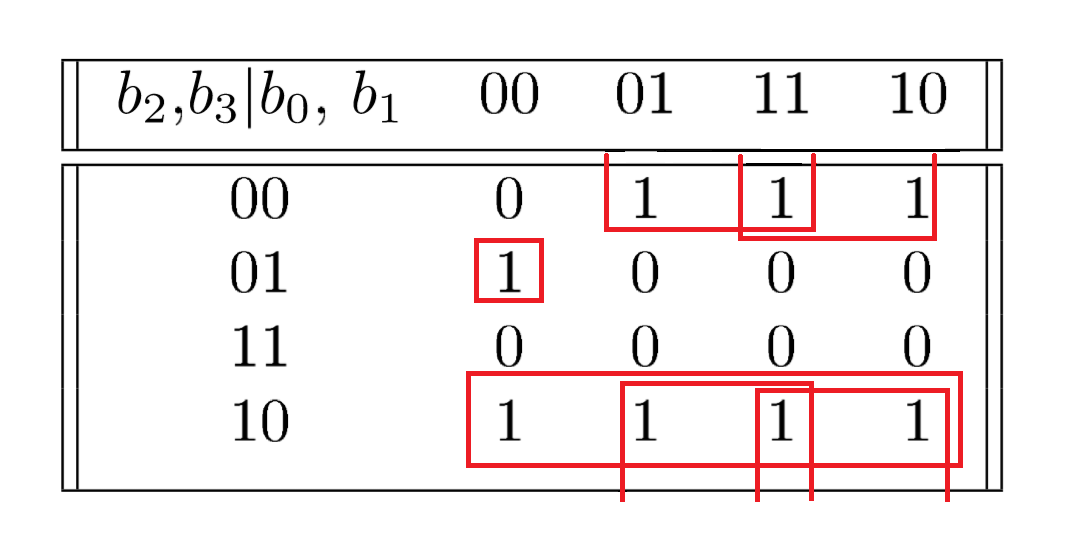
\includegraphics[scale=0.5]{imagenes/karnaugh_mapa_y3.png}
	\caption{Mapa de Karnaugh para $y_3$}
	\label{fig:ej4_karnaugh_mapa_y3}
\end{figure}

%escribo simplificación resultante y_3
De este mapa se puede obtener $y_3$ = $\overline{b_{3}} \cdot b_{2} +\overline{b_{3}}\cdot b_{1} 
+\overline{b_{3}} \cdot b_{0} +b_{3}\cdot \overline{b_{2} \cdot b_{1} \cdot b_{0}} $ 
\par
Así, $y_3$ = $\overline{b_{3}} \cdot (b_{2} + b_{1} + b_{0}) + b_{3}\cdot \overline{b_{2} \cdot b_{1} \cdot b_{0}}$ 

%y_2
\item $y_2$					

\begin{figure}[H]	%Karnaugh para y_2, imagen/tabla
	\centering
	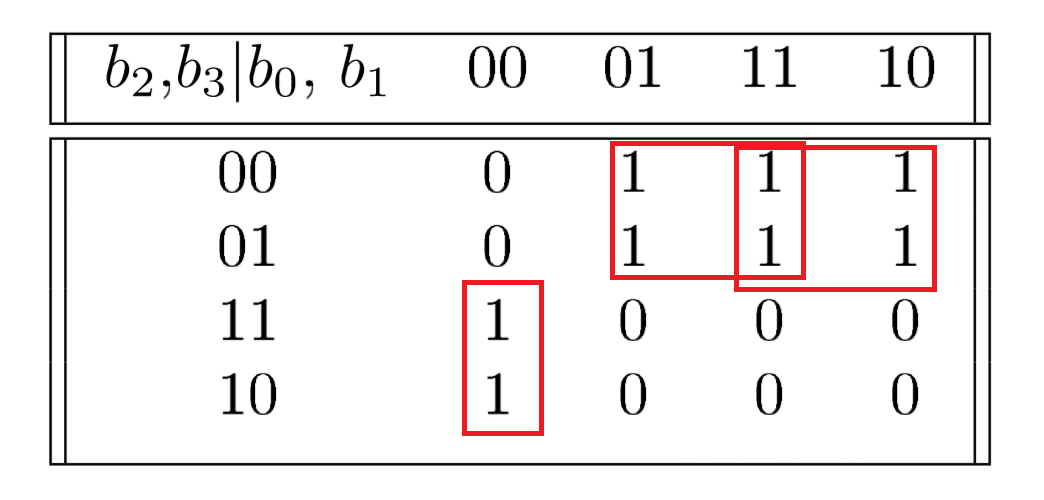
\includegraphics[scale=0.5]{imagenes/karnaugh_mapa_y2.png}
	\caption{Mapa de Karnaugh para $y_2$}
	\label{fig:ej4_karnaugh_mapa_y2}
\end{figure}

%escribo simplificación resultante y_2
De este mapa se puede obtener $y_2$ = $\overline{b_{2}} \cdot b_{1} + \overline{b_{2}} \cdot b_{0} + 
b_{2} \cdot \overline{b_{1}} \cdot \overline{b_{0}}  $ 
\par
Así, $y_2$ = $\overline{b_{2}} \cdot (b_{1} + b_{0}) + b_{3} + b_{2} \cdot \overline{b_{1}} \cdot \overline{b_{0}} $ 

%y_1
\item $y_1$					

\begin{figure}[H]	%Karnaugh para y_1, imagen/tabla
	\centering
	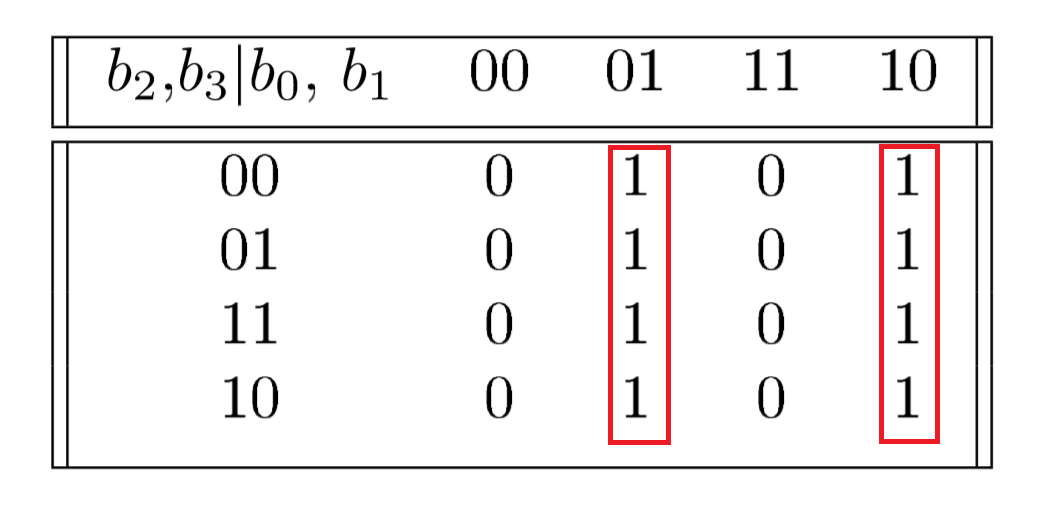
\includegraphics[scale=0.5]{imagenes/karnaugh_mapa_y1.png}
	\caption{Mapa de Karnaugh para $y_1$}
	\label{fig:ej4_karnaugh_mapa_y1}
\end{figure}

%escribo simplificación resultante y_1
De este mapa se puede obtener $y_1$ = $\overline{b_{1}} \cdot b_{0}  + \overline{b_{0}} \cdot b_{1}$ 
\par
Así, $y_1$ resulta ser la xor entre $b_{1}$ y $b_{0}$.

%y_0
\item $y_0$					


\begin{figure}[H]	%Karnaugh para y_0, imagen/tabla
	\centering
	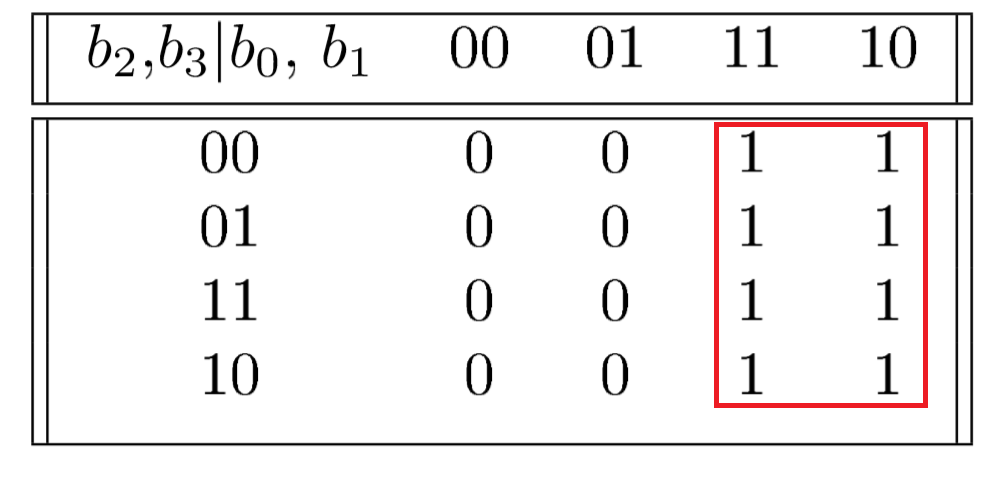
\includegraphics[scale=0.5]{imagenes/karnaugh_mapa_y0.png}
	\caption{Mapa de Karnaugh para $y_0$}
	\label{fig:ej4_karnaugh_mapa_y0}
\end{figure}

%escribo simplificación resultante y_0
De este mapa se puede obtener $y_0$ = $b_{0} $ 
\par
Así, el bit menos significativo de la entrada resulta ser el bit menos significativo de la salida (conexión directa).

\end{itemize} 

\end{enumerate}
 	
\end{document}
